%auto-ignore
\section{Introduction}

One significant challenge in image reconstruction for positron emission tomography (PET) 
involves the suppression of noise, as the emission data collected is highly affected by Poisson noise. 
This is a result of constraints in acquisition duration, the amount of dose that can be injected, 
and the sensitivity of PET scanners. 
In order to reduce the impact of data noise on the image during model-based iterative reconstruction (MBIR), 
various approaches are available. 
One option is to add a "smoothing" prior to the data fidelity term in the cost function being optimized.
In general, we can formulate the resulting optimization problem for any imaging system where the
acquired data follow a Poisson distribution as
%
\begin{equation}
\argmin _{x\geq 0} \sum_{i=1}^{m} \underbrace{(Px + s)_i -  d_i \log \left( (Px + s)_i \right)}_{D_i((Px+s)_i)} + \, \beta R(Kx),
\label{eq:primal} 
\end{equation}
%
where $x$ is the image to be reconstructed, $P$ is the linear forward model, $d$ are the acquired
data and $s$ are additive contaminations.
$\sum_{i=1}^m D_i((Px + s)_i)$ is the negative Poisson log-likelihood, 
$i$ is the index of the data bin and $m$ is the total number of data bins.
In the specific case of time of flight (TOF) PET, $P$ is the time of flight (TOF) PET
forward model including the effects of attenuation, normalization and limited spatial resolution, 
$d$ are the acquired prompt TOF PET coincidences (the emission sinogram), 
and $s$ are the estimated random and scattered coincidences. 

$R(K\cdot)$ is a ``smoothing prior'' consisting of a generic linear operator $K$ that calculates 
local differences and a proper, convex, lower-semicontinous function $R$.
The level of regularization is controlled by the non-negative scalar factor $\beta$.
A specific example for $K$ would be the spatial gradient operator $\nabla$.
Combining the gradient operator for $K$ with the mixed L2-L1 norm for $R$ leads to the well-known 
Total Variation (TV) prior \cite{Rudin1992} or directional TV when using a projected gradient
operators \cite{Ehrhardt2016}.
It was shown that \eqref{eq:primal} can be solved (even for non-smooth priors) using the 
generic primal-dual hybrid gradient (PDHG) algorithm by Chambolle and Pock \cite{Chambolle2011}
or its (much faster) stochastic extension (SPDHG) \cite{Ehrhardt2019} using a subset of the data in every update.

In this work, we summarize our findingings on our proposed listmode extension of SPDHG (LM-SPDHG)
published in \cite{Schramm2022} optimized towards sparse PET emission data such as TOF PET data
from systems with excellent TOF resolution.

\section{LM-SPDHG Algorithm}

As indicated by the name, emission data in listmode format are a chronological list $N$ of detected 
events $e \in N$, where each event is characterized by a small set of (integer) numbers 
(e.g. the number of the two detectors, the discretized TOF difference, and a time stamp).
To process the listmode data during reconstruction without binning it into a sinogram,
we introduce the listmode forward operator $P^{LM}_N$ mapping the image data $x$ to a 
data-vector of dimension $|N|$ via 
%
\begin{equation}
(P^{LM}_N x)_e  = (Px)_{i_e} , \text{ for each }e \in N,
\label{eq:lmop}
\end{equation}
%
where $i_e$ is the sinogram bin in which event $e$ was detected. 
Also, we denote by $s^{LM}$ with $s^{LM}_e = s_{i_e}$ the listmode-based scatter 
and random estimate.

Re-writing the gradient of the negative Poisson log likelihood using listmode data and the
listmode operators is straightforward, such that any gradient-based PET reconstruction algorithm 
can be easily adapted to listmode data.

For a Bayesian approach with prior $R(K \cdot)$ as in \eqref{eq:primal} this is less immediate, 
but we can show that indeed \eqref{eq:primal} can be equivalently re-written into 
a minimization problem involving only the listmode forward operator. 
This allows us to extend the SPDHG algorithm for listmode data and yields the algorithm as shown 
in Algorithm~\ref{alg:lmspdhg}.

\begin{algorithm}[t]
\begin{algorithmic}[1]
\small
\State \textbf{Input} event list $N$, contamination list $s_N$
\State \textbf{Calculate} event counts $\mu_e$ for each e in $N$
\State \textbf{Initialize} $x,w,(S_i)_i,T,(p_i)_i$
\State \textbf{Initialize} list $y_{N} = 1 - (\mu_N /(P^{LM}_{N} x + s_{N}))$ 
\State \textbf{Preprocessing} $\overline{z} = z = {P^T} 1 - {P^{LM}}^T (y_N-1)/\mu_N + K^T w$ %(see \eqref{eq:zinit_lm} and text)
\State \textbf{Split} lists $N$, $s_N$ and $y_N$ into $n$ sublists $N_i$, $y_{N_i}$ and $s_{N_i}$
\Repeat
	\State $x \gets \proj_{\geq 0} (x - T \overline{z})$
	\State Select $i \in \{1,\ldots,n+1\}$ randomly according to $(p_i)_i$
  \If{$i \leq n$}
	  \State $y_{N_i}^+ \gets \prox_{D^*}^{S_i} \left( y_{N_i} + S_i \left(P^{LM}_{N_i} x + s^{LM}_{N_i} \right) \right)$
	  \State $\delta z \gets {P^{LM}_{N_i}}^T \left(\frac{y_{N_i}^+ - y_{N_i}}{\mu_{N_i}}\right)$
	  \State $y_{N_i} \gets y_{N_i}^+$
  \Else
	  \State $w^+ \gets \beta \prox_{R^*}^{S_i/\beta} ((w + S_i  K x)/\beta)$
	  \State $\delta z \gets K^T \left(w^+ - w\right)$
	  \State $w \gets w^+$
  \EndIf
	\State $z \gets z + \delta z$
	\State $\overline{z} \gets  z + (\delta z/p_i)$
\Until{stopping criterion fulfilled}
\State \Return{$x$}
%\EndFunction
\end{algorithmic}
\caption{LM-SPDHG for PET reconstruction}
\label{alg:lmspdhg}
\end{algorithm}


%%%%%%%%%%%%%%%%%%%%%%%%%%%%%%%%%%%%%%%%%%%%%%%%%%%%%%%%%%%%%%%%%%%%%%%%%%%%%%%%%%%%%%%%%%%%%%%%%%%%%%%%%
%%%%%%%%%%%%%%%%%%%%%%%%%%%%%%%%%%%%%%%%%%%%%%%%%%%%%%%%%%%%%%%%%%%%%%%%%%%%%%%%%%%%%%%%%%%%%%%%%%%%%%%%%

\section{Numerical Experiments}

In the absence of an analytical solution to the optimization problems \eqref{eq:primal}, 
we analyzed the convergence of LM-SPDHG and SPDHG with respect to a 
reference solution $x^*$ as done in \cite{Ehrhardt2019}.
Convergence was monitored by tracking the relative cost function
\begin{equation}
c_\text{rel}(x) = (c(x) - c(x^*)) / (c(x^0) - c(x^*)) \ ,
\end{equation}
where $c(x)$ is the cost function to be optimized in \eqref{eq:primal} and $x^0$ is the initialization
used for $x$.
Moreover, convergence was also montiored in image space by tracking the peak signal-to-noise ratio
with respect to $x^*$
\begin{equation}
\text{PSNR}(x) = 20\,\log_{10} \left( \|x^*\|_\infty/\sqrt{\text{MSE}(x,x^*)} \right) \ ,
\end{equation}
where MSE is the mean squared error.
The reference solution was obtained by running the deterministic PDHG (SPDHG without subsets)
for 20000 iterations.
Since running PDHG with 20000 iterations using realistic 3D TOF PET data takes a very long 
time (approx. 250\,h), all numerical convergence experiments were performed using simulated 2D TOF PET data.
A 2D software brain phantom with a gray to white matter contrast of 4:1 was created
based on the brainweb phantom \cite{Collins1998} and used to generate simulated 2D TOF data 
including the effects of limited spatial resolution, attenuation and a flat contamination mimicking 
random and scattered coincidences with a contamination fraction of 42\%.
The geometry and TOF resolution of the simulated 2D PET system was chosen to 
mimic one direct plane of a state-of-the art TOF PET scanner with a ring diameter of 650\,mm
and a 400\,ps TOF resolution.


\section{Results}

\begin{figure}
\centering
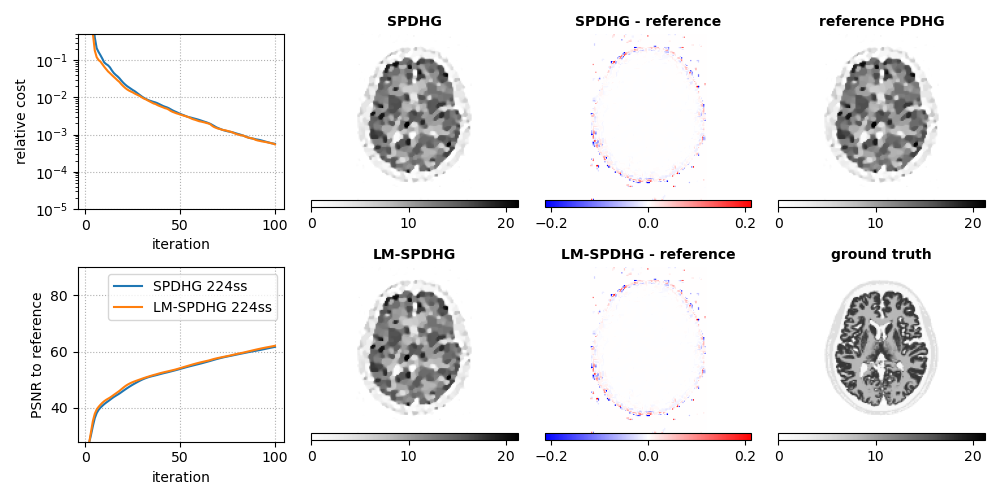
\includegraphics[width=1.0\columnwidth]{./figure3a.png}
\caption{Comparison of convergence of sinogram SPDHG and LM-SPDHG
         for using 244 subsets. 3e5 true (5e5 prompt) counts, TV prior, $\beta = 0.03$}
\label{fig:lm-spdhg-var}
\end{figure}


Figure~\ref{fig:lm-spdhg-var} summarizes the convergence comparison between sinogram SPDHG and 
LM-SPDHG.
As demonstrated by the convergence metrics and the reconstructed images, the convergence of
sinogram SPDHG and LM-SPDHG is almost identical.
This also holds for different count levels and for the structural DTV priors (not shown here).

\begin{figure}
    \centering
    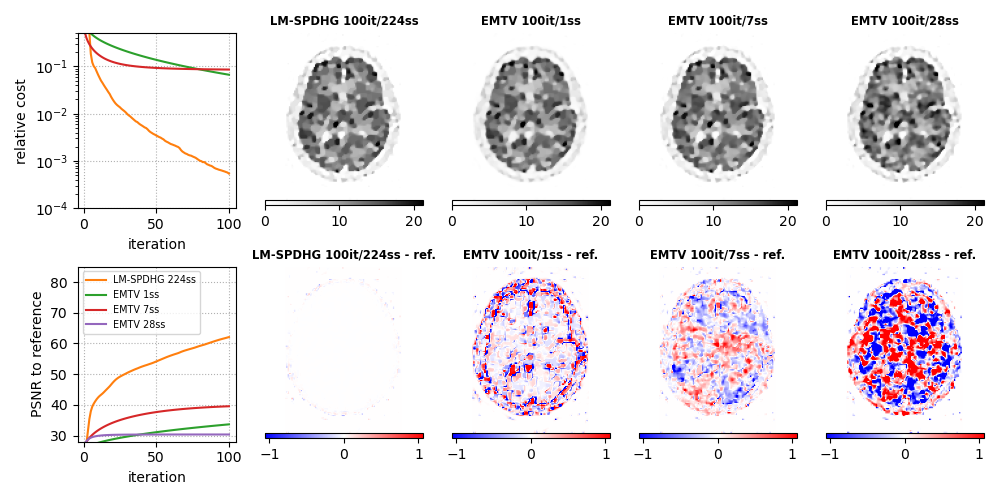
\includegraphics[width=1.0\columnwidth]{./figure4a.png}
    \caption{Same as Fig.~\ref{fig:lm-spdhg-var} but comparing the convergence of LM-SPDHG using
             224 subsets and listmode EM-TV using 1, 7 and 28 subsets 3e5 true (5e5 prompt) counts, TV prior, $\beta = 0.03$}
\label{fig:emtv}
\end{figure}

A comparison between the convergence of LM-SPDHG using 224 subsets and listmode 
EM-TV \cite{Sawatzky2008} using 1, 7 and 28 subsets is shown in Fig.~\ref{fig:emtv}.
In all sub figures, LM-SPDHG converges much faster than EM-TV.
Moreover, when using more than 1 subset, EM-TV seems to remains on a limit cycle.

%%%%%%%%%%%%%%%%%%%%%%%%%%%%%%%%%%%%%%%%%%%%%%%%%%%%%%%%%%%%%%%%%%%%%%%%%%%%%%%%%%%%%%%%%%%%%%%%%%%%%%%%%
%
\section{Discussion and Conclusion}

The results of our numerical experiments presented in this work demonstrate that the speed of 
convergence of LM-SPDHG is essentially the same as the one of the original SPDHG using
sinograms.
For clinical acquisitions with state-of-the-art TOF PET scanners resulting in extremely
sparse data, LM-SPDHG has two distinct advantages compared to SPDHG.
First, during the iterations all forward and back projections can be performed in listmode
which is faster compared to sinogram projectors for sparse TOF data, and, 
second, the memory requirements are substantially reduced since storage of complete
TOF sinograms is avoided.
Note that due to the page limit, results from real 3D TOF data as shown in \cite{Schramm2022}
are not included, but will be presented at the conference.
